%% This document gives an example on how to use the ntnubachelorthesis
%% LaTeX document class.
%% Use oneside for PDF delivery and twoside for printing in a book style
%% use language english, norsk, nynorsk and one of the following shortenings
%%  ``BSP'' Bachelor i Spillprogrammering,\\
%%  ``BRD'' Bachelor i drift av nettverk og datasystemer,\\
%%  ``BIS'' Bachelor i Informasjonssikkerhet,\\
%%  ``BPU'' Bachelor i Programvareutvikling, \\
%%  ``BIND'' Bachelor i Ingeniorfad - data, \\
%%  ``BADR'' Bachelor i drift av datasystemer, \\
%%  ``BIT'' Bachelor i informatikk, \\
%%  ``BABED'' Bachelor i IT-støttet bedriftsutvikling.
%%   for example \documentclass[BIS,norsk,twoside]{ntnuthesis/ntnubachelorthesis}

\documentclass[BSP,english,oneside]{ntnuthesis/ntnubachelorthesis}

\usepackage{csvsimple}
\usepackage{booktabs}
\usepackage{minted}
\usepackage{pdfpages}
\usepackage{graphicx}
\usepackage[]{algpseudocode}

\newcommand{\comment}[1]{\textcolor{blue}{\emph{#1}}}  %% use of the colour and you can see how to use commands with parts \comment{so what}

%% The class files defines these two
%% \newcommand{\NTNU}{Norwegian University for Science and Technology} %

% you can create you one #define like structures using the \newcommand feature
% you can change behaviour using \renewcommand

\newcommand{\com}[1]{{\color{red}#1}} % supervisor comment
%\renewcommand{\com}[1]{} %remove starting % to remove supervisor comments
% This will appear in text \com{Lecuters comment} and be visible unless you uncomment
% the renewcommand line.

\newcommand{\todo}[1]{{\color{green}#1}} % items to do
%\renewcommand{\todo}[1]{} %remove starting % to remove items to do

\newcommand{\n}[1]{{\color{blue}#1}} % other comment
%\renewcommand{\n}[1]{} %remove starting % to remove notes

\newcommand{\dn}[1]{} % add the d to a note to say that you have finished with it.


% Norwegian Characters,  needs the {} or to be separate from the next letters
% \o{}   \aa{}   \ae{}   so at the end of a word you can use \o  \aa   \ae
% \O{}   \AA{}   \AE{}   you can also just leave a space and latex will remove it
%    eg, NTNU i Gj\o vik  or NTNU i Gj\o{}vik

\begin{document}

\thesistitle{Technology Exploration - Unity Entity Component System}
\thesisauthor{Andreas Wang}

\nmtkeywords{Test}
\nmtdesc{
Hello!
}


\nmtoppdragsgiver{\NTNU}
\nmtcontact{Andreas Wang, andrwan@stud.ntnu.no, 48048162}

\thesisdate{\ntnubachelorthesisdate}
\useyear{16.11.2018}

\nmtappnumber{0} %number of appendixes
\nmtpagecount{} %currently auto calculated but might be wrong % this is the file which contains all the details about your thesis

\makefrontpages % make the frontpages

\tableofcontents
\listoffigures
%\listoftables
%\listoflistings

\chapter{Introduction}
The Unity Engine sees a large amount of usage within the indie, mid-budget and VR portions of the game industry. On the other hand, the usage of Unity is less prevalent for AAA development in comparison with competitors like Unreal. So why does Unity not see as much usage in this field? One of the reasons for this related to performance and the control of it. Large portions of Unity are written in C\# which means that memory management is automated. The garbage collector in C\# can for example create unwanted stutters in places where developers do not want them. Furthermore, Unity does not really have any official support for multithreaded code either. It is possible to write multithreaded code using C\# functionality like \emph{async} and \emph{await}, but this approach is limited as interfacing with the Unity API is only possible on the main thread. 

As a means to deal with this, Unity has recently launched their new Entity Component System (shortened to ''ECS'') in conjunction with an interface to Unity's native job system and the new Burst compiler. The goal with ECS is to provide an alternative data-oriented workflow for developers that focuses on performance by default and allowing the developer to focus their optimisations on the data and its processing. ECS is currently in early preview, but it is planned to release in 2019 according to Unity's latest R/D talk at Unite LA~\cite{unityLARND}. It is not production ready by any means as much of the core functionality is not yet implemented. Regardless, given the focus on ''performance by default'' it would be interesting to see how ECS compares to the standard object-oriented form of Unity. 
\section{Background}
* Background - what was the approach previously
  * Assembly was used a lot initially
  * Working in straight C is also an option
  * Games nowadays often make use of object oriented design.
* Before detailing what Unity ECS is, it might be useful to provide some context on the underlying design philosophy it makes use of: Data-Oriented Design

\subsection{Data-Oriented Design}
* There are a fair amount of resources discussing data-oriented design, this section is mostly a summary from Noel's blogpost on it. http://gamesfromwithin.com/data-oriented-design

* What is the problem with object-oriented design in game development?
   * Cache misses are problematic
      * It is expensive and takes a lot of CPU cycles to deal with
      * Technicalities are discussed here http://www.dataorienteddesign.com/dodmain/node17.html (written by Richard Fabian)
      * Object-oriented patterns in general can very easily result in cache misses for games
   * Multithreaded code is very error-prone and synchronisation can be costly. 
* What is data-oriented design and how does it fix the problem? 
   * A shift in focus from objects to pure data
      * "The type of data, how it is laid out in memory and how it will be read + processed in the game" (Citation from link)
      * Decoupling data from logic
   * By breaking objects into components and grouping components of the same type together it is a lot easier to sequentially process them compared to the object oriented approach of dealing with each object and its related hierarchies in isolation. 
   * As a result it works well on large groups of objects/things(?)
   * Data-oriented design makes it easier to write parallel code
      * we are mostly dealing with input data, a small function that processes it and some output data. (Large amounts of SIMD style instructions)
      * less synchronisation is generally needed
   * Performance benefits
    * The same code is executed over and over in a data-oriented system which results in efficient use of instruction caches
    * Data caches are also efficiently used since data of the same type are stored in large contiguous blocks and are sequentually processed. 
    * In terms of optimisation we also primarily have to think of data usage and processing at a higher level which can be hard with traditional OOP
   * Other benefits
    * Code is often more modular as we mostly have to write small functions that transform some data
       * These small functions generally have little dependency on other parts of code
       * No need to understand complex hierarchies to understand the basics of the code
   * A drawback with DOD though is that it is different from what most people are used to so it takes time to rethink and restructure how we think about code architectures. 
   * While data-oriented design primarily is used for games, there has also been a case for using it outside of this domain https://www.youtube.com/watch?v=yy8jQgmhbAU
\subsection{Unity ECS, Job System and Burst}
  * What is Unity ECS?	
	* A paradigm shift from object oriented design to data oriented design.
	* In standard Unity the architecture is as follows
		* A scene consists of GameObjects
		* GameObjects contain components which can be seen as data containers or scripts with behaviours attached.
	* In general, GameObjects are rather heavyweight and come with a Transform component by default.
		* There are a lot of different callbacks per GameObject with MonoBehaviour components attached
	* Unity has previously tried to provide more lightweight versions of GameObjects through ScriptableObjects.
		* These are primarily used as data containers with potentially some minor behaviour code.
        * Everything still is tied to GameObjects though as ScriptableObjects have to be loaded and worked with in a component that exists within a gameobject. 
    * ECS
    	* Shifting how Unity works from the core to allow for better performance by default.
    	* Instead of GameObjects we now have Entities which could be seen as a more lightweight version of the former. 
    	   * An entity in this case is ultimately just an ID to a list of components
    	* Components still exist in ECS, but they are purely used as data containers with no behaviour.
    	* Any behavioural code is instead handled by Systems which process groups of component data, following the same principles we see in data-oriented design
    		* I.e. instead of having three GameObjects with a "IdentifyAndShootPlayer" script that are run individually per gameobject we now have a System that works on all Entities that contain "IdentifyAndShootPlayerComponent".
    	* This data oriented paradigm is by default a fair bit faster than the standard Unity approach as a good amount of overhead is decreased and cache usage is improved.
        * This is also very well suited as a multithreaded environment.
    * Job System
      * Allowing developers to write multithreaded code by providing access to the native Job System that the engine uses internally (Cite I guess?).
	  * Closely coupled with ECS to parallelise how Systems work on Components, but can also be used in Standard Unity. 
      * Tries to avoid common pitfalls in multithreading by being architectured in a way that avoids race conditions.
    * Burst Compiler
      * A compiler that compiles a subset of C\# called "High Performance C\#" for better performance. 
    * Making use of these three in tandem is generally what is recommended for highest performance gains. 
    * Everything is currently in early preview so you are expected to write all the Systems yourself outside of barebones graphics and transform handling. 
	* The goal for Unity is to provide a ECS equivalent to everything that currently exists in the engine today. (Cite?) 
	* The general workflow for writing a parallel System is similar to working with a GPU where your Job is similar to that of a Shader in terms of how you need to declare everything you want to use ahead of time and how you are limited in interfacing with the outside world

\subsection{Resources for learning about Unity ECS, Job System and Burst Compiler}
* Sources:
  * Search terms which find good resources related to the technology
     * Unity forums have their own section for ECS where a lot of questions, discussion and similarly can be found
  * Links to a good explanations
     * Gotchas link (useful for new developers that are trying to get used to ECS. It probably is a bit outdated though as ECS syntax and functionality changes fairly quickly based on feedback and the fact that it still is in early preview. It was useful for me when I was learning ECS during last summer, but it might be less useful now)
  * Links to a good resources/tutorials
     * ECS repo documentation and sample code
     * Unity's official tutorials
     * As with any documentation or tutorials, they might be slightly outdated from the latest bleeding edge build of ECS, but the core concepts should of course stay the same. 
     * Some small useful technical utilities
        * https://coffeebraingames.wordpress.com/2018/10/14/some-ecs-utility-scripts/
\section{Methods}
\subsection{Test Cases and Data Acquisition}
Testing was divided into three baseline cases:
\begin{enumerate}
    \item A naive Unity implementation
    \item A job optimised version of the naive Unity implementation
    \item A naive Unity ECS implementation
\end{enumerate}
These three were then further optimised on an individual level to see how far I could get them in terms of performance. In general, the goal for making these test cases was to create a scenario where there are a large amount of moving objects on screen. This is something data-oriented design excels at in theory and it would be interesting to see how big the differences are. 

Data acquisition consisted of a 30 second recording where the frame latencies in milliseconds were collected per frame. This recording was initiated a few seconds after the program had started in order to not include spikes from the start-up. This data was then output to a .CSV file which was uploaded to the project spreadsheet on Google Sheets~\cite{projectSpreadsheet}.

\subsection{Choice of Galaxy Sizes}
The choice of galaxy size for the baseline cases was determined by a few decisions. The minimum size of any galaxy was 10 000 stars as going below this resulted in a somewhat uninteresting visual simulation. Outside of this, the size of the galaxy was largely dependent on overall performance of a test case. The general goal was to have a galaxy at a size that would result in approximately 60 frames per second. The reasoning for this is that taxing the hardware could make the bottlenecks in the software more apparent. This was rather important since I had limited experience with optimisation before going into this project.  

\subsection{Testing Environment}
The testing environment on the hardware side consisted of:
\begin{itemize}
    \item Intel Core i7-6700k CPU
    \item nVidia GeForce GTX 1080 GPU
    \item 16 GB RAM
\end{itemize}

The testing environment on the software side consisted of:
\begin{itemize}
    \item Windows 10 OS - Build 1809
    \item Unity Engine - Version 2018.2.7f1
    \item Unity Entities Package - Version 0.0.12-preview.16
    \item Unity Editor Viewport Resolution of 1047x589
\end{itemize}

\subsection{Determining the Next Course for Optimisation}
I primarily relied on test results and profiler data to determine bottlenecks that could see improvement. This consisted of looking for irregular frame latency spikes and seeing how much time the engine spent on all the elements in a average frame. After determining an area that could use optimisation I started to look up resources for how this could be done before implementing the changes. 

\subsection{Usage of Framerate/Frame Latency Display and In-Editor Testing}
While testing the application, a real-time frame rate and latency display was used in order to get an overview of the general performance~\cite{graphy}. The reason for using a third party display for this is that Unity's own framerate and latency counters are inaccurate. The inaccuracy comes from the fact that the values are inflated to what the engine estimates the program will manage in release mode and not inside the editor~\cite{forumFramerateStats}. This estimation can be incorrect and as such, it has limited value. As an example: Unity's Stats window could for example show that the ECS test case ran at 200 frames per second, while it in reality ran at 68 frames per second. 

Given that ECS is not production ready yet, building the project for release also seemed to actually decrease performance of the ECS cases. This was not directly recorded, but it seemed like the performance dropped by at least 20 frames per second in release mode compared to running in the editor. Due to this, all tests were performed in-editor with the related overhead that this brings. 
\section{Implementation}
The project repository containing all of the source code from the project can be found here~\cite{projectrepo}.

\subsection{Initial Plan for Testing}
Originally, the plan was to compare pathfinding between standard Unity and the ECS version as a new AI API by Unity allows ECS to interface with it. This was scrapped fairly early on as there was too little documentation on how the new AI API worked so I could not get anything to run properly. Instead, I moved on to a simpler test scenario with transform manipulation for visual effects. The original pathfinding code still exists in the project repository, but it is not used.

\subsection{Transform Management Using a Galaxy Simulation}
\subsubsection{Simulation Design}
The design of the simulation consists of two parts: 
\begin{enumerate}
    \item Spawning and distributing stars across the galaxy
    \item Making each star orbit around the center of the galaxy at a given speed
\end{enumerate}
Stars are spawned in a manner that results in larger densities of stars towards the center of the galaxy and lower densities towards the outer edges. This is handled by defining a number of orbit circles and the difference in radius between them. The same amount of stars are then spawned per orbit, although a small random value is applied so that the galaxy looks more noisy and not like a set of circles. The general pseudocode for the spawning process looks like this:

\begin{algorithmic}
\For {$i=0; i<numberOfOrbits; i++$}
    \For{$j=0; j<numberOfStars/numberOfOrbits; j++$}
         \State Spawn Star at galaxyPosition;
         \State Generate a random point at the edge of a unit circle;
         \State Create normalized direction from random point;
         \State Star.position = galaxyPosition +
         \State (direction * (i+1) * distanceBetweenOrbits * randomValue);
         \State Star.orbitSpeed = starDistanceToGalaxyCenter;
    \EndFor
\EndFor
\end{algorithmic}

After the spawning process, each star then orbits around the center of the galaxy with a speed that is relative to the distance between the star and the center of the galaxy. The orbit speed has to be variable as keeping it the same would make it look like there is static galaxy that simply rotates around. This is because there are no real physics at play here and only a calculation for translating position on the edge of a circle using angles. To provide an example: with a speed modifier of 1 a star at (0,0,1) and a star at (0,0,100) would have moved to (1,0,0) and (100,0,0) with a 180 degree angle change when the galaxy is perpendicular to the Y-axis. 

\subsubsection{The Representation of Stars and Post Processing Usage}
Each star makes use of the default sphere mesh in Unity in combination with a randomly selected material which supports GPU instancing. This should provide a more taxing (and visually interesting) environment compared to simply using two dimensional sprites. 

Only having a large amount of differently coloured spheres would not look particularly appealing in a galaxy. This is why post processing bloom is applied in combination with HDR emission in the material of the stars to create a glowing appearance. As a result, the larger concentration of stars towards the center of the galaxy produces far more glow which provides a more visually natural image since stars actually emit light. The visual difference between not using and using bloom can be seen in Figure~\ref{fig:nobloom} and~\ref{fig:bloom}.
Multi-sampling anti aliasing (MSAA) is applied as it mitigates the flickering that comes from moving objects with bloom(TODO: Does this need citation? It's mostly just an artifact of Unity's bloom implementation). Finally, temporal anti aliasing (TAA) is applied to smooth the final image. 

\begin{figure}[tbph]
    \centering
    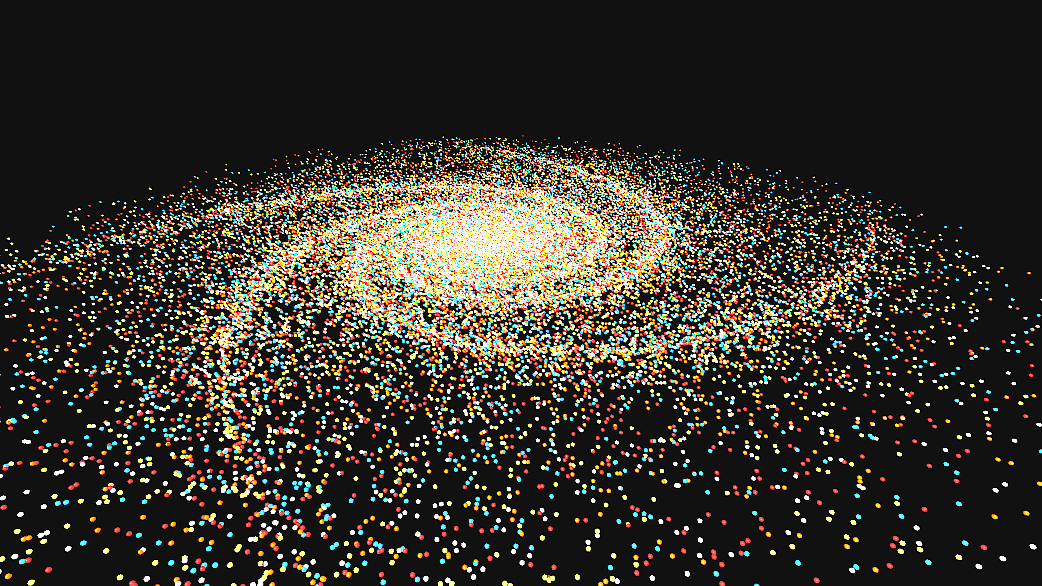
\includegraphics[width=1\textwidth]{Figures/noBloom.png}
    \caption[Galaxy without bloom]{The appearance of the simulated galaxy without any bloom}
    \label{fig:nobloom}
\end{figure}

\begin{figure}[tbph]
    \centering
    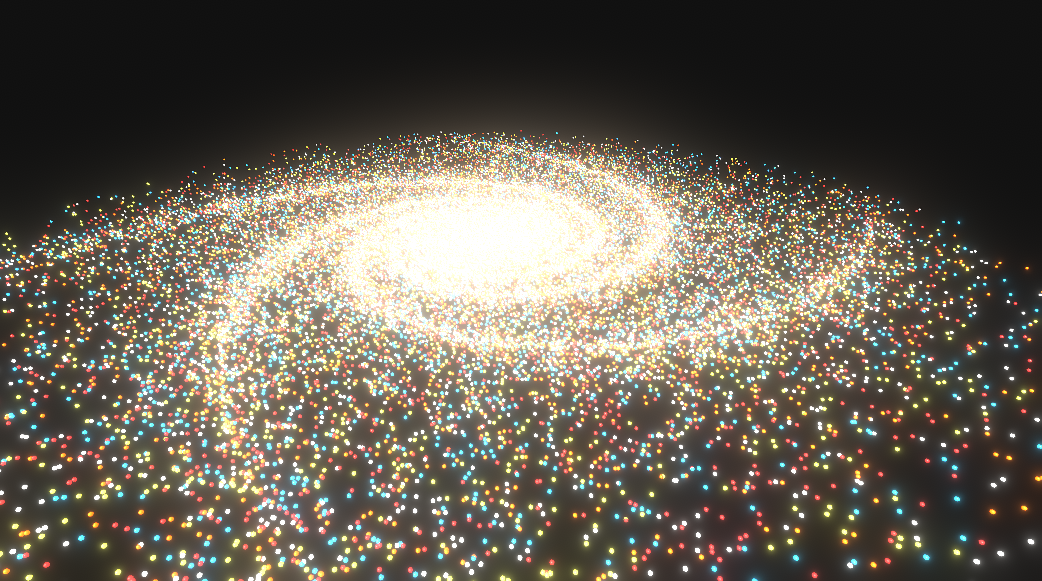
\includegraphics[width=1\textwidth]{Figures/bloom.png}
    \caption[Galaxy with bloom]{The appearance of the simulated galaxy with bloom}
    \label{fig:bloom}
\end{figure}

\subsubsection{Naive Unity Implementation}
The naive Unity implementation is split in two source files: StarSpawner.cs~\cite{naiveSpawner} and OrbitAroundTransform.cs~\cite{naiveOrbiter}. The former takes care of spawning stars from a provided prefab in a similar vein to the previously mentioned pseudocode. The latter script is attached to every single star and consists of a target to orbit around, the axis that the rotation makes use of and the speed of rotation. This script also has a Update() method which rotates the star around the center of the galaxy using Unity's RotateAround() function~\cite{rotateAroundFunction}.

This is more or less the simplest implementation I think of, hence the naming of the case. Since each star has a script attached which inherits from Unity's MonoBehaviour class, the performance of this test case is expected to be rather low.

\subsubsection{Job Optimised Unity Implementation}
The job optimised counterpart to the naive Unity implementation consists of one source file: GalaxyManager.cs~\cite{jobOptimizedManager}. The script takes care of both spawning and translating the stars around. This means that each star does not contain any behaviour by itself and everything is managed in one script that exists in one instance. 

The process of spawning stars is more or less the same as with the naive implementation, although the distance between the star and the center of the galaxy is stored for later usage. 

The process of translating stars is handled by using a job from the new Job System that Unity introduced together with ECS and the Burst compiler. This is a ParallelFor-style job, meaning that it will split the loop among all available worker threads. The job is designed to be similar with how Unity's RotateAround() function~\cite{rotateAroundFunction} is in terms of usage, although it does not change any rotation matrices. One thing to note about the Job System is that all data that is used should be declared and provided ahead of time so the job can execute it in a native environment. Due to this, there is some additional boilerplate code in this test case so that all important data can be stored and transferred over to the job. 

The means of translating a star along its own orbit is handled by first finding the current angle between the star and the center of the galaxy. This angle is then subtracted from with Time.deltaTime multiplied by the speed of the star. Standard trigonometry functions like cosine and sine are used together with the new angle to update the position of the star relative to the galaxy center. Finally, the star is offset so that it keeps the distance from the center which was stored during spawning. 

\subsubsection{Naive ECS Implementation}
The ECS implementation is split up into a variety of files and the general pipeline is fairly different from standard Unity. This section is mostly focused on the specific implementation in this case so some technical background in ECS might be useful to understand the source code. The naming of the test case is mostly a result of the fact that I could not really think of many other ways to implement the logic in ECS.

\paragraph{Components and Bootstrapping}
Since the galaxy simulation only consists of stars there only is one component. This can be seen in the TransformOrbitComponents.cs script~\cite{transformOrbitComponent} where the OrbitingStar component only stores the necessary data for orbiting. Entity creation is handled in a bootstrapper script~\cite{bootstrapper} which consumes galaxy settings from a GameObject in the scene and creates entities that consist of four components. These four components are Position, Scale, OrbitingStar and a MeshInstanceRenderer. During creation of entities, each star is placed around in the galaxy similar to how the other test cases handle it. 

\paragraph{Systems}
This implementation only consists of one system which is found in StarOrbitSystem.cs~\cite{orbitSystem}. The algorithm for translation is mostly the same as in the job optimised Unity case although there is a difference in how data is acquired. This is handled with a IJobProcessComponentData$<$...$>$-style job which specifically works with ECS components. Providing component types as parameters to this interface results in the job filtering all entities based on the provided input. In this case, the job acquires all entities that contain a Position and OrbitingStar component and handles translation of these. 

\section{Results}
* Plenty of data~\cite{projectSpreadsheet}
* Link to videos to demonstrate the technology
* Will probably present the combined latency diagram for each case and end with the overview of average FPS

\subsection{Overview of Search Space}
\begin{figure}[tbph]
    \centering
    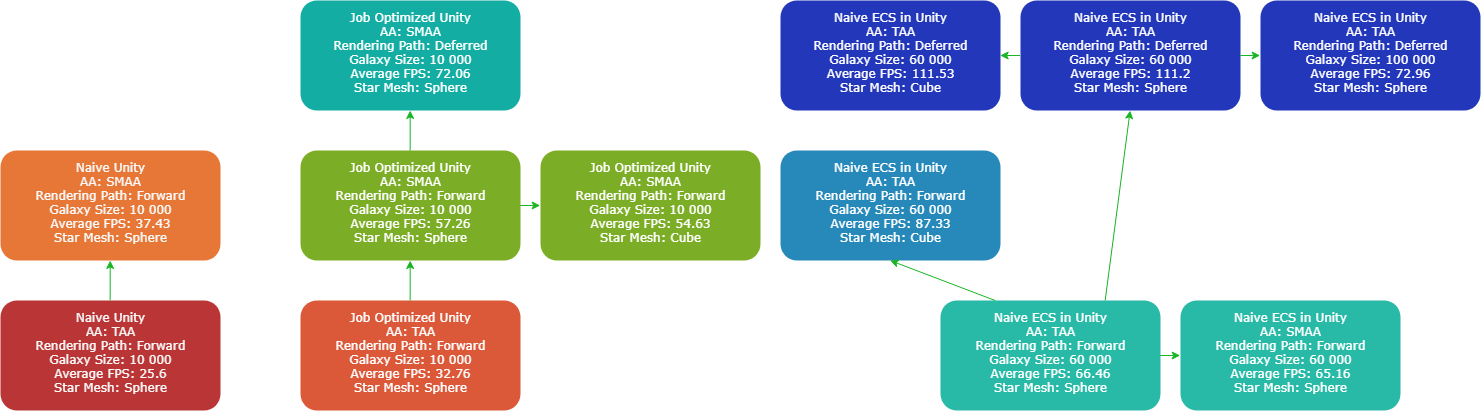
\includegraphics[width=1\textwidth]{Figures/SearchSpace.png}
    \caption[Optimisation Search Space And Combinations]{The space of optimisations that were measured}
    \label{fig:searchspace}
\end{figure}
\chapter{Discussion}
\section{Discussion Per Test Condition}
   * Discussing the decisions I made for how to optimise further from the base test cases (Generally a per test discussion)
      * Graphics was a bottleneck
            * Graphics Performance guides from Unity looked at
                  * Tried various proposals from link
   * Profiler frames discussion 
      * Tradeoffs for Deferred Rendering in this case
         * Flickering, can look at 60k and 100k videos
         * It is not highly noticeable here, but the fewer stars there are the more flicker there is
         * It is generally up to the developer whether they find the tradeoff worth it in their case. The performance boost is rather substantial at least
\subsection{Naive Unity}
\subsection{Job Optimised Unity}
\subsection{Naive ECS}

\section{Overall Discussion of Results}
* Differences in bottlenecks
         * Standard Unity is heavily affected by AA, while ECS is not
         * Mesh complexity matters a lot for ECS in a forward rendering scenario, but not for standard Unity
            * When using deferred rendering this difference is neglible

   * While both Job Optimised Unity and ECS are parallel how come the difference in performance is still so big?
      * Partly on the architectural side
         * Object oriented design vs. data oriented design
         * With a lot of GameObjects the cache usage is pretty bad due to always moving around in different hierarchies per object
         * The entity component system model leverages the benefits of data-oriented design in this regard and makes better use of cache
         * On the rendering side, while both interface with the same graphics API, there are some differences in how data is structured and sent to the GPU which further could improve performance
      * The ECS version is also compiled with the Burst compiler.
         * I was originally under the impression that Burst only worked with ECS, but it seems like it now supports the Job System in general. 
         * So it might be possible to further improve the performance of the joboptimised Unity condition by adding burst compilation
         * You should probably not expect too big of a difference though as burst primarily is meant to work in synergy with ECS and the Job System

\section{Reliability of Test Results}
      * Moving pieces that are hard to control
          * While trying out the same test conditions at different times a frame rate variance of around 5-8fps was observed
          * Operating System impact on performance
             * Can be a result of the operating system having different degrees of load on the hardware at different times.
             * For all the tests, I tried to keep any additional programs closed, but the OS can still do things in the background that impact performance
          * Editor overhead
             * Should generally be consistent between tests, but this is hard to fully confirm
      * Overhead from framerate counter should not matter much as this is consistently in use for all tests
      
      * The ECS and Job optimised cases could be more affected by OS related interrupts as all available threads are working during runtime and might be problematic with context switching
      * The naive unity case mostly runs on the main thread so it is less affected by this problem

\section{Unrecorded Test Cases}
   * Other test cases on additional variables that were briefly looked at, but not recorded due to time constraints 
      * Assuming the average framerate and stability stayed more or less the same between a pre change and post change execution of the program
   * Editor vs. Release
      * Mentioned in Methods
      * Very strange how performance drops so drastically in release mode, even when actual resolution is similar or the same between editor/build
      * Not necessarily easy to find out why
         * My performance measurer only works with the editor due to differences in folder structure
      * Speculation: 
         * Specific quality settings that only apply in release mode might result in lower performance
         * Burst and ECS have specific optimisations that only work in debug so far
   * Resolution
      * Can look at the provided videos relative to the performance benchmark as those have a maximised viewport
      * Expect some additional overhead from actually recording though
   
\section{Code Complexity vs. Performance Payoff}
   * Code complexity vs performance payoff
       * Halsteadt's complexity/Cyclomatic Complexity could be looked at
   * This test environment is not particularly complex
      * The complexity of Pure ECS might explode quite a bit for larger projects
         * Comparatively large amounts of monobehaviour usage struggles with performance in larger projects
         * So it is all a balancing act
      * Hybrid solutions can be useful in that regard
   
\section{The Future of Unity ECS} 
* The Future:
  * What is the expected lifetime of this technology? (Depends on user feedback, but generally it seems to be something Unity Technologies wants to coexist with the existing architecture so developers can either choose or use hybrid solutions)
  * What might replace it in the future? (''nothing'' unless the way our CPU's are architectured changes drastically so data oriented design is less beneficial :p)

\section{Conclusion}



\bibliographystyle{ntnuthesis/ntnubachelorthesis}
\bibliography{IMT4888}

\appendix %after this line all chapters will have letters instead of numbers
% spreadsheet data?

\end{document}